% ------------------------------------------------------
% File    : cruz_computing_2020.tex
% Content : Article for Computing
% Date    : 30/03/2020
% Version : 2.0
% Authors : M. Cruz, A. Durán
% ------------------------------------------------------

% ------------------------------------------------------
% Last update: 30/03/2020 (Amador)
% Limpieza de restos previos.
% ------------------------------------------------------
  
\documentclass[smallextended]{svjour3}	% onecolumn (second format)
\usepackage[utf8]{inputenc}	% UTF-8 character set 
\usepackage[english]{babel}	% this paper is written in English
\usepackage{cruz_other} % other packages and definitions

% Insert the name of "your journal" with
\journalname{Computing}

% The correct dates will be entered by the editor
\date{Received: date / Accepted: date}

\begin{document}

\title{\TITLE\thanks{\FUNDING}}
 %\subtitle{Do you have a subtitle?\\ If so, write it here}
\titlerunning{\SHORT}       

\author{%
  Margarita Cruz      \and
  Beatriz Bern\'ardez \and
  Amador Dur\'an      \and
  Cathy Guevara     \and
  Antonio Ruiz{\--}Cort\'es
}

\authorrunning{M. Cruz et al.} % if too long for running head

\institute{%
Margarita Cruz \at \email{cruz@us.es} 		 				\\ \\
Beatriz Bern\'ardez \at \email{beat@us.es} 				\\ \\
Amador Dur\'an \at \email{amador@us.es}		 				\\ \\
Cathy Guevara \at 
\email{cguevara@utn.edu.ec}
%Universidad Técnica del Norte: Ibarra, Imbabura, EC
% carrera de Ingeniería en Sistemas Computacionales (Facultad de Ingeniería en Ciencias Aplicadas)
\\ \\
Antonio Ruiz{\--}Cort\'es \at \email{aruiz@us.es} \\
\at
Department of Computer Languages and Systems, Universidad de Sevilla, Seville, Spain
}

\maketitle

% ------------------------------------------------------
% File    : acronyms.tex
% Content : Acrónimos 
% Date    : 15/3/2019
% Version : 1.0
% Authors : M.Cruz
% ------------------------------------------------------
% Usar \gls{SE}
\newacronym{SE}{SE}{Software Engineering}
%\newacronym{NS}{NS}{Natural Science}
\newacronym{SC}{SC}{Science}
\newacronym{AUT}{AUT}{Automatic experiments}

\newacronym{ESE}{ESE}{Empirical Software Engineering}
\newacronym{DSR}{DSR}{Design Science Research}

\newacronym{AI}{AI}{Agronomic Engineering}
\newacronym{ETSIA}{ETSIA}{E.T.S. Ingeniería Agronómica}
\newacronym{ETSII}{ETSII}{E.T.S. Ingeniería Informática}
\newacronym{IG-CSIC}{IG-CSIC}{Instituto de la Grasa}
\newacronym{IRNAS-CSIC}{IRNAS-CSIC}{Instituto de Recursos Naturales y Agrobiología de Sevilla}
\newacronym{RQs}{RQs}{research questions}

\newacronym{EX}{EX}{controlled experiment}
\newacronym{QE}{QE}{quasi--experiment}
\newacronym{CS}{CS}{case study}
\newacronym{SV}{SV}{survey}

\newacronym{Mind}{Mind}{A family of experiment on Mindfulness}
\newacronym{Req}{Req}{A family of experiment on Requirements Analysis}
\newacronym{Code}{Code}{A family of experiment on Code Evaluation Techniques}

%\newcommand{\SE}{SE\xspace}
\newcommand{\SoftEng}{SoftEng\xspace}
\newcommand{\Mind}{Mind\xspace}
\newcommand{\Req}{Req\xspace}
\newcommand{\Code}{Code\xspace}

%\newcommand{\SC}{SC\xspace}
\newcommand{\Science}{Science\xspace}
\newcommand{\Soil}{Soil\xspace}
\newcommand{\Quality}{Quality\xspace}
\newcommand{\Bio}{Bio\xspace}
\newcommand{\Olive}{Olive\xspace}
\newcommand{\Diet}{Diet\xspace}

%\newcommand{\AUT}{AUT\xspace}
\newcommand{\Automatic}{Automatic\xspace}
\newcommand{\Testing}{Testing\xspace}
\newcommand{\SPL}{SPL\xspace}


\newcommand{\Expressiveness}{Expressiveness\xspace}
\newcommand{\expressiveness}{expressiveness\xspace}
\newcommand{\Precision}{Precision\xspace}
\newcommand{\precision}{precision\xspace}
\newcommand{\Understandability}{Understandability\xspace}
\newcommand{\understandability}{understandability\xspace}
\newcommand{\Traceability}{Traceability\xspace}
\newcommand{\traceability}{traceability\xspace}
\newcommand{\Usability}{Usability\xspace}
\newcommand{\usability}{usability\xspace}
\newcommand{\applicability}{applicability\xspace}




%\newcommand{\SI}{SI\xspace}
%\newcommand{\AI}{AI\xspace}

\newcommand{\DSR}{DSR\xspace}
%\newcommand{\etal}{\emph{et al}.\xspace} 
%\newcommand{\SCOPUS}{SCOPUS\xspace}

%\newcommand{\EX}{EX\xspace}
%\newcommand{\SV}{SV\xspace}
%\newcommand{\CS}{CS\xspace}
%\newcommand{\QE}{QE\xspace}
 
 





% -------
% Content
% -------

% ------------------------------------------------------
% File    : cruz_2020_00_abstract.tex
% Content : Abstract section of the article 
% Date    : 16/07/2018
% Version : 1.0
% Authors : M. Cruz
% ------------------------------------------------------
% ------------------------------------------------------
% Last update: 22/11/2020
% ------------------------------------------------------

\begin{abstract}
\emph{Context}: Replication of empirical studies in Software Engineering is necessary to consolidate acquired knowledge and generalize results from related studies. To reap the benefits of replications, information must be published in a way that allows a better understanding of the differences between the replication and the baseline study. %
%
\emph{Objective}: 
The goal of the present work is to facilitate documentation of replication changes and, therefore, the replicability of experiments in Empirical Software Engineering. %
%
\emph{Method}: First, a meta--model was presented to formalize related concepts and a template with linguistic patterns was designed to visually display the meta--model information. 
Based on the proposed template, the CÆSAR tool was developed to facilitate the definition of changes and provide an overview of the family of experiments.
The template was evaluated by specifying changes in replications of several families of experiments in a multiple--case study encompassing various areas of knowledge and types of experiments. The application of the template in other areas has made possible to analyze the difficulties encountered and compare the terminology and concepts used.
\emph{Results}: 
By means of the multiple--case study, the expressiveness, precision, usability and traceability of the proposed template have been analyzed. 
The limitations encountered have allowed the template to evolve from its initial version and, in spite of the different terminology and concepts used in the area of sciences, the improved template has allowed to define changes systematically and homogeneously. 

\keywords{%
Replication \and 
Meta--model \and 
Template 		\and 
Linguistic patterns \and
Empirical study     \and 
Family of experiments}

\end{abstract}
% ------------------------------------------------------
% File    : cruz_computing_2020_01_introduction.tex
% Content : Introduction (y DSR) section of the article for Computing
% Date    : 1/12/2018
% Authors : M.Cruz
% ------------------------------------------------------

% ------------------------------------------------------
% Last update: 26/10/2020 (Marga)
% - Cambios a partir de la tesis.
% ------------------------------------------------------

\section{Introduction}
\label{sec:intro}

\gls{ESE} allows the evaluation of new methods, techniques and tools to know the convenience of using them during the development process  \cite{sjoberg2005survey}.
Once an artefact has been evaluated for the first time, the study needs to be replicated in different contexts and conditions, not only to consolidate the acquired knowledge, but also to know if its results can be generalized \cite{Baldassarre}.
First, it is advisable to carry out internal replications, then external ones which are those carried out by other experimenters and are the ones with the greatest power of confirmation. Without external replications the results are only provisional \cite{brooks1996replication}.

However, despite the importance of replications, and although the practice of replications has increased in recent years  \cite{da2014replication}, the number of replications in \gls{SE} remains low  \cite{solari2017content}.
Among the causes influencing this situation are, on the one hand, the lack of agreement on common criteria for reporting replications \cite{carver2010towards}.
On the other hand, \emph{tacit knowledge} not explicit in the replication report \cite{shull2002replicating}. In addition, there is a lack or incompleteness of the \emph{laboratory packages} that are necessary to facilitate replications \cite{solari2017content}. All this, together with  the effort and resources needed to carry out an experiment \cite{da2014replication}.

When considering a new replication, the need to incorporate changes to the original experiment arises for several reasons: \emph{i)} \emph{to avoid propagating problems} from the original experiment \cite{kitchenham2008role}; \emph{ii)} \emph{to adapt the replication} to different conditions where the original experiment was carried out \cite{Baldassarre}; and \emph{iii)} \emph{to generalize the results} of the original experiment  \cite{shull2008role}. 

The importance of properly specifying changes in replications is twofold: on the one hand, for the author of the first replication himself; he must deepen in the nature of the proposed changes and analyze their repercussion, determining their convenience in the design of the experiment and their effect on a possible meta-analysis.
It will be necessary to analyze its influence on the validity of the experiment and to document the reason for this change.
On the other hand, for successive replications, before proposing new changes, it will be very helpful to know the changes already made in order to know how an original experiment has evolved within a family of experiments and why the changes have been made. This facilitates the design of experiments, without repeating failures already identified and adapting the experiment to the new environment with more success. 

Within the documentation to be published on the replications, Carver's \emph{guidelines} \cite{carver2010towards} highlight the need to describe these changes with respect to the original experiment and the situation that caused the change. In \cite{gomez2014understanding}, changes are classified according to the element of the experimental configuration affected by the change and related to the purpose of replication.
Several guidelines for the reporting of controlled experiments have been proposed in \gls{SE} \cite{jedlitschka2008reporting,juristo2013basics,wohlin:experimentation}. 
However, to the best of our knowledge, there is only the initial proposed Carver guidelines \cite{carver2010towards} for the publication of replications of experiments.
 

This paper proposes an approach for specifying changes that tries not only to report the changes but to design and deepen in the proposed changes. It is based on: \emph{i}) a meta--model to formalize information requirements; and \emph{ii)} a template that facilitates reusability, visual representation and avoids redundancies \cite{duran1999requirements,del2016using}. 

To validate the proposal, the template has been empirically evaluated through a multiple--case study using the CÆSAR tool developed to facilitate the definition of changes.
We think that the systematic specification of changes will support the process of replication of controlled experiments

% ----------------------------
% File    : T-DSR.tex
% Content : Tabla DRS
% Date    : 1/12/2018
% Version : 1.0
% Authors : M.Cruz
% ----------------------------
\begin{table*}
  \caption{Activities of the \DSR methodology and corresponding sections}
  \label{tab:fases-DSR}
  \centering
  \scriptsize
  \begin{tabularx}{0.98\textwidth}{
    >{\hsize=0.4\hsize}X
    >{\hsize=0.9\hsize}X
    >{\hsize=0.23\hsize}X}
 
    \toprule
    Actividad  &
    Descripción   &
    Sección \\
    \midrule
    
    \emph{Problem identification and motivation}  &
    Need to address an accurate definition of changes for the reporting of replications of controlled experiments & 
    \ref{sec:intro}  \\ 
    
    \emph{Solution objectives definition}  & 
    Facilitate documentation of changes so that they are clearly specified. Literature is reviewed to: i) analyse how changes are being reported; ii) identify the information involved; and, iii) know other proposals &
    \ref{sec:SLR} \\
    
    \emph{Design and Development}  & 
    A meta--model is proposed. A possible implementation of the meta--model is the template completed with L-patterns & 
    \ref{sec:metamodelo}, \ref{sec:plantilla} \\
    
    \emph{Demonstration}  &
    The first version of the template is instantiated by defining the changes of a family of experiments belonging to the \gls{SE} area.  &
    \ref{sec:Mind} \\
    
    \emph{Evaluation}  &
    The artefact, in our case the template, is evaluated in a multiple case study encompassing various areas of knowledge and types of experiments. CÆSAR tool is used as a proof of concept. & 
    \ref{sec:Case},  \ref{sec:SoftEng-Case}, \ref{sec:Science-Case}, \ref{sec:Automatic-Case} \\
    
    \emph{Communication} & 
    The results of the research are published &  \\ 
    
    \bottomrule
  	\end{tabularx}   
\end{table*}

\gls{DSR} has been adopted as a research methodology. \gls{DSR} creates and evaluates \emph{artefacts} in order to solve \emph{identified organizational problems} \cite{von2004design}. The phases followed in our research are those defined in the DSR methodology proposed in \cite{peffers2007design}. \tablename~\ref{tab:fases-DSR} shows these phases and their correspondence with the sections of this work.

 The remainder of this paper is organized as follows:  Section  \ref{sec:metamodelo} presents the meta--model on which the template is based;  Section \ref{sec:plantilla} proposes the template for the specification of replication changes; Section \ref{sec:Case} presents our multiple--case study; Sections \ref{sec:SoftEng-Case}, \ref{sec:Science-Case} and \ref{sec:Automatic-Case}  present each of the case study individually; Section \ref{sec:trabajos} analyses the related work; and Section \ref{sec:conclusions} presents the concluding remarks and future work.

% ------------------------------------------------------
% File    : cruz_computing_2020_02_background.tex
% Content : Introduction (y DSR) section of the article for Computing
% Date    : 19/11/2020
% Authors : M.Cruz
% ----------------------------------------------

\section{Background}
\label{sec:background}

Before presenting our proposal, it is first necessary to point out the importance of replications and then to introduce some concepts used to specify the replications.

To justify the importance of replications, below are some organisations that have published or taken an interest in the subject of replications and its related aspects.

In \cite{acm}, the Association for Computing Machinery (ACM) recommend that three separate badges related to artifact review be associated with research articles and classifies them as: \emph{i) artifacts evaluated}, \emph{ii) artifacts available} and \emph{iii) results validated}. In these last ones, the same results have been obtained in a subsequent study conducted by people other than the authors. Two levels are distinguished: \emph{results reproduced} and \emph{results replicated}, depending on whether or not the artifacts provided by the author are used.

ACM stresses that an experimental result is not fully established unless it can be independently \emph{reproduced}, noting furthermore, the benefits obtained by making research artifacts available to the public to facilitate replications that verify the robustness of the original results.

Similarly, at ICSE (International Conference
on Software Engineering) it is noted that reviewing the artifacts of accepted papers increases the likelihood that the results can be  \emph{replicated} and \emph{reproduced} by other researchers. 
ICSE invites the authors of accepted contributions to present the associated artefacts for evaluation and to receive one of the ACM badges.  Authors can also make short presentations at the ROSE (Recognizing and Rewarding Open Science in Software Engineering) festival. ROSE festivals are held at major conferences in the area.

Finally, to highlight the \emph{Open Science} initiative to make research data public, thereby increasing the \emph{transparency} and \emph{reproducibility} of the studies \cite{fernandez2019open}.
\emph{Open Science} is based on: \emph{i)} open access to the articles, \emph{ii)} open data and \emph{iii)} open source software.

% --- Dimensiones ---

Concerning the specification of replications, it is necessary to go deeper into the nature of the changes involved. 
A change can affect an element of the experimental configuration. It is necessary to identify the elements that make up the experimental configuration and which of these elements can be changed and still be considered as the same experiment.
In \cite{gomez2014understanding}, elements of the experimental configuration are classified into the following groups called dimensions: \textit{Operationalization}, \textit{Population}, \textit{Protocol} and \textit{Stakeholder}. 
There is also a fifth \emph{Context} dimension identified by us.

In a controlled experiment, there are the constructs of \emph{cause} and \emph{effect} (or also called independent and dependent variables).
The \textit{Operationalization} dimension includes the translation of the \emph{cause} and \emph{effect} constructs into their concrete manifestations.
The \emph{treatment} is the \textit{Operationalization} of the \emph{cause}.
\emph{Metrics} and \emph{measurement} procedures are the \emph{operationalization} of the \emph{effect}.

The \emph{Population} dimension includes the \emph{experimental subjects} that act on the experimental \emph{objects}. 
The treatments are applied to the combination of \emph{objects} and \emph{experimental subjects}.

The \emph{Protocol} dimension is the configuration of \emph{experimental design}, \emph{experimental material}, \emph{guides}, \emph{iv) measuring instruments} and \emph{data analysis techniques} to observe a particular effect.

The \emph{Stakeholder} dimension includes the researchers participating in the experiment in their different \emph{roles: designer, analyst, trainer, monitor} and \emph{ measurer}.

In this article, the \emph{Context} dimension related to the environment in which the experiment is carried out is proposed. Changes in the context affect the results.
For example, carrying out the replication at a different time or day may affect the results or carry it out at exam time instead of at the beginning of the course. 


% ------------------------------------
% File    : cruz_computing_2020_03_metamodel.tex
% Content : Meta--model section of the article for Computing
% Date    : 1/12/2018
% Authors : M.Cruz
% ------------------------------------
% ------------------------------
% Last update: 1/11/2020 (MCruz)
% Actualización a partir de la tesis
% ------------------------------
 
%-----------------------------------
\section{Meta--model about replications and changes}
\label{sec:metamodelo} 
%-----------------------------------

The information involved in the replication is detailed below and will serve as the basis for the definition of the meta--model.

First, to identify both the replication and the baseline experiment a code or \emph{acronym} relative to the baseline experiment is used. The baseline experiment can be either an original experiment or a previous replication.

Next, it is necessary to provide a general idea of the experiment. It seems reasonable to record the \emph{Goal--Question--Metric (GQM)} \cite{Basili1994} or, failing that, the \emph{goal}. 
A brief \emph{description} of the experiment will also be recorded, along with its \textit{site} and \textit{date} of performance.

Regarding replication, in addition to data concerning the context (\textit{site} and \textit{date} of replication), it is relevant to identify the \textit{type} and \textit{purpose} of replication.

Depending on who carries out the replication, these are classified as \textit{internal}, carried out by the original experimenters, and \textit{external}, carried out by independent experimenters.

The replication \textit{purpose} can be: \emph{i) Confirm results} \emph{ii) Generalise results} and \emph{iii) Overcome some limitations of the baseline experiment}.

Next, we focus on identifying information related to the specification of the \textit{changes} that characterise the replication.
That is, for each change, the \emph{situation in the baseline experiment and in the replication} along with the \emph{cause of change} are described.

Next, depending on the \emph{element of the experimental configuration} modified, changes can be classified into \emph{dimensions}: 
%Gómez \etal \cite{gomez2014understanding} define the following \emph{dimensions}:

\begin{itemize}
    \item \textit{Operationalization}. Includes changes related to the elements: \emph{i) cause} (e.g. changes in the application of treatment), \emph{ii) effect} (e.g. changes in metrics) and \emph{iii) measurement procedure}.
    
    \item \textit{Population}. The element affected by the change is some property of the subjects or experimental units (e.g. experimental subjects with different experience level or age from the baseline experiment). The modified \emph{property} will be identified.
    
    \item \textit{Protocol}. Includes changes related to the elements: \emph{i) experimental design}, \emph{ii) experimental material} (e.g. changes to the code of the program to be inspected), \emph{iii) guides} (e.g. changes to the instructions provided), \emph{iv) measuring instruments} (e.g. changes to the questionnaire for data collection)  and \emph{v) data analysis techniques}. The experimental protocol is the set up of these elements to observe the effects of treatments \cite{Juristo2012}.

    \item \textit{Stakeholder}. Related to changes in the roles of experimenters. The elements are: \emph{i) designer}, \emph{ii) analyst}, \emph{iii) trainer}, \emph{iv) monitor} and \emph{v) measurer}.
    
    \item \textit{Context}. The element affected by the change, is a \emph{context variable} that will be necessary to identif. %y (e.g. perform the baseline experiment at the beginning of the course and the replication at exam time).
    
\end{itemize}    

Likewise, each \emph{change} may affect one or more types of \emph{threats to validity} \cite{wohlin:experimentation}:

\begin{itemize}
    \item \emph{Conclusion validity}. Related to obtaining correct conclusions about the relationship between the \emph{treatment} and the \emph{result} of an experiment.
    
    \item \emph{Internal validity}. Assures that the result is caused by the \emph{treatment} and is not a consequence of other factors.
     
    \item \emph{Construct validity}. Assures that the treatment reflects the \emph{construct} of the \emph{cause} and  that the \emph{outcome} reflects the \emph{construct} of the effect.
    
    \item \emph{External validity}. Related to the generalization of the results outside the scope of the study.
\end{itemize}

Once the information about the replications and their changes has been conceptualized, a meta--model is proposed for its representation.
Fig.~\ref{fig:Metamodelo-UML} depicts the current version of meta--model using UML class diagram notation.

%-----------------------
\begin{figure*}[h]
    %\centering
    \includegraphics[width=\textwidth]{Metamodelo}
    \caption{Meta-model of replications and changes}
    \label{fig:Metamodelo-UML} 
\end{figure*}
%-----------------------

% ----------------------------------
% File    : cruz_computing_2020_04_template.tex
% Content : Template section of the article for Computing
% Date    : 1/12/2018
% Authors : M.Cruz
% ----------------------------------

% ----------------------------------
% Last update: 10/11/2020 (MCruz)
% Actualización a partir de la tesis
% ----------------------------------

%----------------------------------
\section{Template for specifying changes in replications}
\label{sec:plantilla}
%----------------------------------

This section develops a possible visual representation of the meta--model through a template. 
The template has a double purpose: on the one hand, it motivates the researcher to make the change and its details explicit (reducing \emph{tacit knowledge}) and, on the other hand, it helps the reader to better understand the replication and to follow the trace of how the original experiment evolves in the succession of experiments across a family of them.

The template is completed with L-patterns. They are common phrases identified and parameterized for some fields in the template \cite{duran2002supporting}.
In the notation used to describe the L-patterns, words or phrases between \textless \hspace{0.5 mm} and \textgreater \hspace{1 mm} must be properly replaced.
Words or phrases between \{ and \} and separated by \textbar \hspace{1 mm} represents options, only one option must be chosen.
Words between [ and ]$^+$ are repeated 1 or more times; that is, they appear at least once but there may be more than one occurrence
and between [ and ] are optional.

Filling the blanks in pre–written sentences, i.e. L–patterns, is easier and faster than writing a whole paragraph. 

%-----------------------
\begin{figure*}[h]
    %\centering
    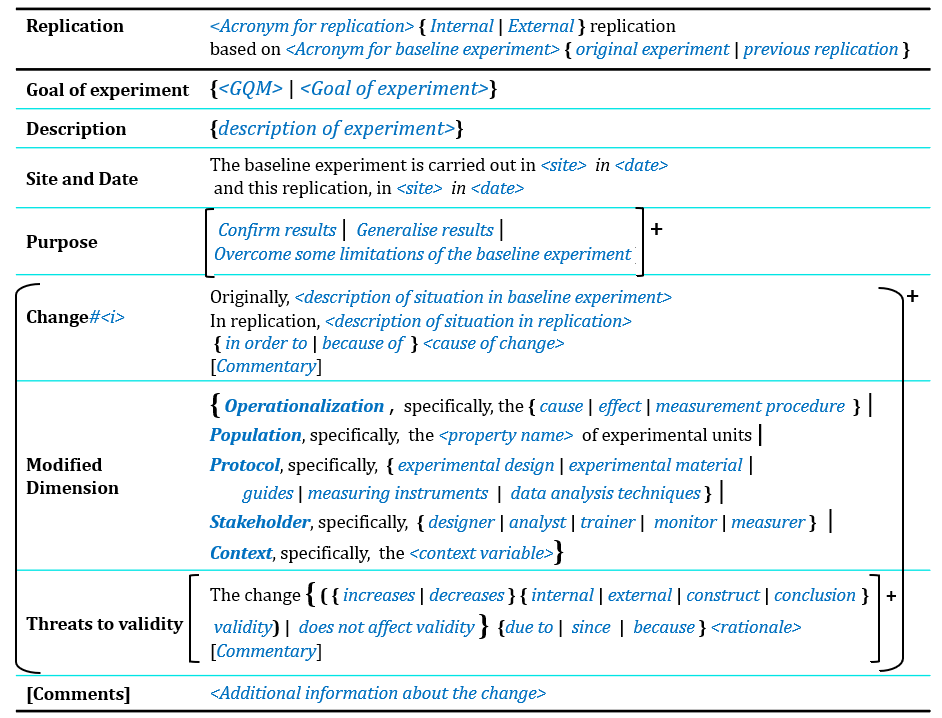
\includegraphics[width=1\textwidth]{figures/Template.png}
    \caption{Template to specfy changes in a replication}
    \label{fig:Template-V1} 
\end{figure*}
%-----------------------



Fig.~\ref{fig:Template-V1} shows the proposed template.
The template consists of two clearly differentiated parts: a general part for the specification of \textit{basic aspects} of replication and a specific part for each of the \textit{changes} included in the replication.


% ----------------------------------------
% File    : cruz_2020_05_caseStudy.tex
% Content : Multiple--Case Study section of the article for Computing
% Date    : 1/Julio/2019
% Version : 2.0
% Authors : M.Cruz 
% ----------------------------------------

% -----------------------------------
% Last update: 16/11/2020 (MCruz)
% Actualización a partir de la tesis
% -----------------------------------

%-----------------------------------------------------------
\section{Evaluation of the Template. Multiple--Case Study}
\label{sec:Case}
%-----------------------------------------------------------

Case study is a research methodology that is carried out in its natural context. Studies range from well--organised studies to small examples in a university lab \cite{runeson2009guidelines,runeson2012case}.
\emph{Multiple--case study} includes more than one case with different characteristics. If the information obtained is similar, conclusions are more solid \cite{runeson2012case}.  

We carried out a multiple--case study that includes three case studies with the main objective of evaluating the use of the template by specifying changes in the replications of selected families in three different settings.

The research method followed in this study has been based on case study research process proposed in Runeson and H{\"o}st \cite{runeson2009guidelines} and Runeson \etal \cite{runeson2012case}. 

To carry out the validation, the CÆSAR tool, developed by the authors of this paper and based on the proposed template, has been used to manage replication changes.
It has been developed using the Grails\footnote{https://grails.org/} framework on Groovy\footnote{https://groovy-lang.org/}.

The current prototype consists of three main views that allow: \emph{i)} to describe the base experiment and its replications, \emph{ii)} to specify the changes of each replication and \emph{iii)} to identify the threats to validity involved in each change.

The tool is available at https://metamodelo.herokuapp.com/. 
We are working to make the tool evolve as an assistant so that experimenters can define their replications and changes, automatically generating the \LaTeX \xspace code corresponding to the template. 

%-----------------------------------------
\subsection{Multiple--Case Study phases}
\label{sec:CS-design}
%-----------------------------------------
As shown in Fig.~\ref{fig:Multiple-CaseStudy} three main phases are identified, namely: \emph{i) Case study design}, \emph{ii) Plan, collect and analyse} and \emph{iii) Joint analysis and report}.

%------------------------------
\begin{figure}[htbp]
    \centering
    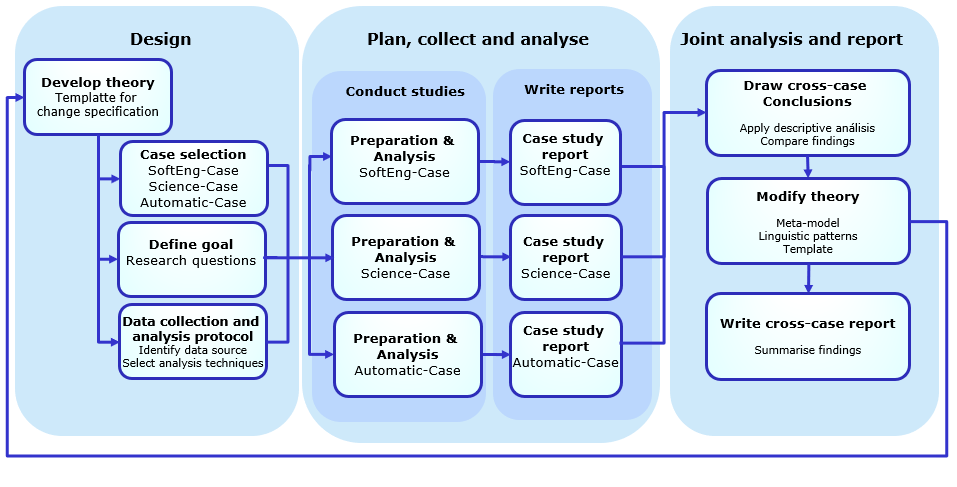
\includegraphics[width=0.9\textwidth] {figures/Multiple-Case}
     \caption{Phases of multiple--case study based on \cite{runeson2012case}}
    \label{fig:Multiple-CaseStudy} 
\end{figure}
%-------------------------------

In the first phase, \emph{case studies} have been selected and \gls{RQs} have been proposed:

%--------------------
%  Case selection
%--------------------

\begin{itemize}   
    \item \emph{Case study in Software engineering} \emph{(\SoftEng-Case)}. Initially, three families belonging to the \SE area that deal with: \emph{i) Mindfulness} (\emph{\Mind}), \emph{ii) Requirements analysis} (\emph{\Req}) and \emph{iii) Code evaluation techniques} (\emph{\Code}) were selected. 
        
    \item \emph{Case study in science} \emph{(\Science-Case)}. Afterwards, and to evaluate the usefulness of the template in other areas of knowledge, four families belonging to \emph{\Science} area and dealing with: \emph{i) Decontamination of soils} (\emph{\Soil}), \emph{ii) Quality analysis of virgin olive oil} (\emph{\Quality}), \emph{iii) Extraction  of  olive oil components} (\emph{\Olive}) and \emph{iv) Influence of diet on cholesterol accumulation} (\emph{\Diet}) were selected.
     
    \item \emph{Case study in \Automatic experiments} \emph{(\Automatic-Case)}. Finally, to evaluate the template in other types of experiments such as algorithmic experiments or those running simulations, two families of experiments on: \emph{i) Automated software testing} (\emph{\Testing}) and \emph{ii) Software Product Line testing} (\emph{\SPL}) were selected.
\end{itemize}
    

%--------------------
%  Define goal
%--------------------
In order to analyse the \emph{\expressiveness, \precision, \usability} and \emph{\traceability} of the proposed template, the following set of \gls{RQs} has been enunciated: 
   
\begin{itemize}
    \item RQ1: \emph{\Expressiveness}. What proportion of changes has it been possible to define?
    Is the \expressiveness of the template greater than other guidelines followed?

    \item RQ2: \emph{\Precision}. Through L--patterns, is the definition of changes more precise than in natural language or tables? Does it detect missing information?

    \item RQ3: \emph{\Usability}. Which fields of the template have presented understanding problems?
    Are the researchers familiar with the terminology? 
   
    \item RQ4: \emph{\Traceability}. By recording changes using the template, does it facilitate \emph{\traceability} between replications?
        
\end{itemize}
   

The second phase includes the preparation for data collection and the analysis.

%-----------------------
%  Preparation for data 
%-----------------------

According to Lethbridge et al. \cite{lethbridge2005studying} \emph{data collection techniques} can be divided into three degrees: \emph{i)} first degree of data collection techniques requires \emph{direct access} to a participant population, \emph{ii)} second degree implies \emph{access to participants environment} as they work, and \emph{iii)} third degree requires \emph{access only to work artifacts}. 
    
\begin{itemize}
    \item In \emph{\SoftEng-Case}, first family has been carried out by some of the authors of the present study. In the remaining families, the templates have also been filled by us, reading the studies that report the replications.
	
    \item In \emph{\Science-Case}, several meetings have been held with researchers belonging to the \emph{E.T.S. Ingeniería Agronómica (ETSIA)} and \emph{Instituto  de la Grasa (IG-CSIC)}. The goal of this meetings were: \emph{i)} To present and explain the use of the template; \emph{ii)} To ask each researcher to select an experiment --advised by us-- with at least one replication and, if possible, has been published; \emph{iii)} Collect the opinion of the researchers once the template has been filled in by the replication author; and \emph{iv)} Answer a questionnaire to check whether the terminology used is the same as \gls{SE}. Each template was filled in by the replication author.
    
    \item In \emph{\Automatic-Case}, researchers belonged to \gls{SE} knowledge area and they already knew the template.  The procedure was similar to the previous case. 
    Templates were filled in by us and validated by replication authors. They also answered a questionnaire about the terminology used in \emph{\Automatic experiments} and we collected their opinion.
\end{itemize}
    
\emph{Data collection techniques} from all three grades have been used:
    \emph{i)} opinions on the use and usefulness of the template have been collected through questionnaires and semi--structured interviews in the researchers' workplaces. (first and second degrees); and \emph{ii)} in order to select the families of experiments, we have used \emph{archival data}; we have reviewed the main publications of the researchers involved. \emph{Archival data} is a type of third--degree data that can be collected in a case study.   

Once the template has been completed, it is analysed whether the fields that have not been filled in are due to the different terminology used or to the lack of the required information. %
It is also analysed whether the template collects all the information that the researcher needs to reflect.
In order to fully interpret the application of the template, details such as who filled in the template (e.g. replication authors), how it was filled in (e.g. from the replication report), when it was filled in (e.g. after the replication was carried out) or whether the template was validated once filled in, are of interest.
     
\tablename~\ref{tab:compara-Case} summarizes the families of each case study along with their number of replications and changes. 
In total, the template has enabled 95 changes to be specified corresponding to 24 replications within 9 families of experiments. 
     
The complete instantiation of the replications that constitute the multiple--case study using the template, is available at the laboratory package at https://exemplar.us.es/demo/...

Table \ref{tab:template-Soil}  shows the specification of the \emph{Soil-2018} replication and its first 5 changes. \\
% ------------------------------------------------------
% File    : T-NS-Soil.tex 
% Content : Replication Soil-2018 (Carmen2018.tex)
% Date    : 2/4/2019
% Version : 1.0
% Authors : C.Florido and M.Cruz
% ------------------------------------------------------
\begin{table*}[h]
    \caption{Specification of the first 5 changes of Soil-2018 replication using the template}
  
    \label{tab:template-Soil}
    \centering
	\scriptsize

    \begin{tabularx}{\textwidth}{
        >{\hsize=0.3\hsize}X
        >{\hsize=0.7\hsize}X}
  
    \toprule

    Replication & 
    \textbf{\emph{Soil-2018}}   Internal replication based on \textbf{\emph{Soil-2016}} original experiment  \\
	
	\midrule   
     
    Description of experiment & 
        To evaluate the effect of a bio-surfactant on the assisted phytoremediation of contaminated soil \\  
 
    Site and Date & 
        The base experiment was carried out in  \textit{ETSIA-University of Seville}  in  \textit{October 2016} and this replication, in  \textit{ETSIA-University of Seville} in \textit{March 2018} \\
    
    Purpose  &  
        Generalise results \\  

\hline   
%-------------------------- 
    Change \textit{1}   & 
        \textbf{Originally}, the experiment was carried out in a cultivation chamber. \\& \textbf{In replication}, was carried out in a greenhouse \\& \textbf{In order to} simulate natural conditions \\
    
    Modified Dimension & 
        \textbf{Population}, specifically, 
        the soil type of the experimental unit soil \\
    
    Threat to validity  & 
        The change increases the external validity \\
        & since it allows to generalize the results carrying out the replication in conditions closer to natural ones \\  

\hline
%-------------------------- 
    Change \textit{2}   & 
        \textbf{Originally}, two plants were used: \emph{Hordeum vulgare} L. and \emph{Brassica juncea} L. \\& \textbf{In replication}, only \emph{Brassica juncea} L. was used \\& \textbf{Because} in the original experiment it was demonstrated that only \emph{Brassica juncea} L. was a metal accumulator plant\\  

    Modified Dimension & 
        \textbf{Protocol}, specifically experimental material \\   
        
    Threat to validity  & 
        The change does not affect validity  \\  
        
\hline
%-------------------------- 
    Change \textit{3}   & 
        \textbf{Originally}, there were two types of soil: Coria (pH=7.8) and Constantina (pH=5.5) \\& \textbf{In replication}, only Constantina soil was used \\& \textbf{Because} it was demonstrated that in the soil of Coria the metal was strongly adsorbed and the phytoextraction did not affect the biomass production   \\  
    Modified Dimension & 
        \textbf{Protocol}, specifically experimental material \\   
    
    Threat to validity  & 
        The change does not affect validity  \\  
        
\hline
%-------------------------- 
    Change \textit{4}   & 
        \textbf{Originally}, Copper (Cu) doses were 0, 500 and 1000 mg $kg^{-1}$ \\& \textbf{In replication}, Cu doses were adjusted to 0, 125, 250 and 500 mg $kg^{-1}$     \\ 
        & \textbf{Because of} Cu doses of 1000 mg $kg^{-1}$ was toxic to the plant \\  
 
    Modified Dimension & 
        \textbf{Operationalization}, specifically independent variable dosisCu \\
        
    Threat to validity & 
        The change increases internal validity because the Cu dose is adjusted to non-toxic levels for the plant \\ 

\hline
%-------------------------- 
    Change \textit{5}   & 
        \textbf{Originally}, Cu was applied as Copper Nitrate \\& \textbf{In replication}, Cu was applied as Copper Sulfate \\
        & \textbf{Because of} is more accessible and the concentrations applied do not affect the plant \\  
 
    Modified Dimension & 
        \textbf{Protocol}, specifically experimental material \\
        
    Threat to validity  & 
        The change does not affect validity  \\  
 
\bottomrule
%	\noalign{\smallskip\smallskip}\hline
	\end{tabularx}  

\end{table*}

% ------------------------------------------------------
% File    : T-Compara.tex
% Content : Compara los experimentos y replicaciones 
% Date    : 2/8/2019
% Version : 1.0
% Authors : M.Cruz
% ------------------------------------------------------
\begin{table*}[h]
    \caption{multiple--case study Summary}
    \label{tab:compara-Case}
    \centering
    \footnotesize
    \begin{tabularx}{\textwidth}{
        >{\hsize=0.4\hsize}X
        %{\hsize=0.28\hsize}X
        cccc}

	 \toprule
  
	Case study & Family & References 
	& No. replications & No. changes \\


     
	\noalign{\smallskip}\hline\noalign{\smallskip}
%    \midrule
	
 	SoftEng-Case 
 		& Mind (Mindfulness)&	
 		\cite{bernardez2014controlled,bernardez-jss-2016} 
 		& 2 & 4 \\
 		
 		& Req  (Requirements) &		
 		\cite{aranda2016estudio} 
 		& 8 & 33 \\

 		& Code (Code Evaluation) & 		\cite{juristo2003functional,juristo2012comparing,juristo2013process}
 		& 4 & 21 \\
 		
  	 	\hline
    	$\sum$ ( \textbf{SoftEng-Case}) & \textbf{3} & & \textbf{14} & \textbf{58}   \\
    	\hline
    
    Science-Case
 		& Soils (Decontamination)$^1$&	
 		\cite{madrid2016fitoextraccion,carvajal2016efecto} 
 		& 2 & 16 \\
 		
 		& Quality (Quality of Oil)$^1$&	
 		
 		& 2 & 4 \\
 		
 		& Olive  (oil components)$^2$ &		
 		\cite{garcia2016extraction}
 		& 1 & 11 \\

 		& Diet (Influence of diet)$^2$ & 					
 		\cite{pacheco2008meal} 		
 		& 1 & 1 \\
 	
	 	\hline
    	$\sum$( \textbf{Science-Case}) & \textbf{4} & &  \textbf{6} &  \textbf{32}  \\
    	\hline
    	
    Automatic-Case
 		& Testing (Testing)&	
 		\cite{parejo2016multi}
 		& 3 & 3 \\
 		
 		& SPL (Product Line)&	
 		\cite{sanchez2014comparison}
 		& 1 & 2 \\
 		
 		\hline
    	$\sum$( \textbf{Automatic-Case}) & \textbf{2} & &  \textbf{4} &  \textbf{5}  \\
    	\hline
    	
    		\hline
    	$\sum$ & \textbf{9} & &  \textbf{24} &  \textbf{95}  \\
    	%\hline
    
    
	\bottomrule
\multicolumn{3}{l}{$^1$E.T.S. Ingeniería Agronómica}  \\
%\multicolumn{3}{l}{$^2$Instituto de Recursos Naturales y Agrobiología}  \\
\multicolumn{3}{l}{$^2$Instituto  de la Grasa}  \\
	  
	\end{tabularx}  
\end{table*}
%\end{table}


In the third phase, conclusions are drawn and limitations encountered have allowed the template to evolve from its initial version.

%--------------------------------
\subsection{Multiple--case studies results}
\label{sec:CS-Results} 
%--------------------------------

\begin{itemize}
%----------------------
%  RQ1: Expressiveness
%---------------------- 
    \item[•] RQ1: \emph{\Expressiveness}. It is analyzed from two aspects:
	
	\begin{enumerate}
        \item  When defining the replications of the first \SoftEng-Case with the initial version of the template, limitations were detected due to the inability to express: 
    
        \begin{itemize}
	        \item Site and date of the baseline experiment and its replication.
	        \item Description of the experiment.
	        \item Acronym for baseline experiment and replication.
	        \item Replications on a previous replication.
	        \item \emph{Validity threats} affecting some changes.
	        \item Changes affecting context variables.
	        \item The cause of the change is unknown.
        \end{itemize}

    After the adjustments, the current version of the template has allowed to express the replications of the families belonging to the three \emph{case studies} and specifically all their changes. 

    \item On the other hand, it is of interest to analyse the \emph{\expressiveness} of the template with respect to other proposals followed by the authors of replications, such as \cite{carver2010towards,wohlin:experimentation,jedlitschka2008reporting,juristo2013basics,runeson2009guidelines}:
    
    \begin{itemize}
        
	    \item \emph{Purpose of the experiment}. In all guidelines, it is recommended to report the \emph{purpose of the experiment}. 
	
	    \item \emph{Changes to the baseline experiment and its cause}. Only in Carver's guidelines \cite{carver2010towards} --the only specific guidelines for replication-- is it recommended to report the \emph{changes} along with the causes. Similarly, Juristo and Moreno \cite{juristo2013basics} when referring to previous experiments, recommend to indicate \emph{the altered characteristics}.
	
	    \item \emph{Validity threats}. Another of the issues that should be addressed in the experiment report are the \emph{threats to validity}. It's mentioned in all the guidelines except Carver's.
	    
	    \item \emph{Use of L-pattern}. It is not used in any guide. The use of L-patters facilitates the definition of change and therefore increases \emph{\expressiveness}.

    \end{itemize}

    The proposed template include both the \emph{purpose} for carrying out the replication and the definition of the change together with the specific \emph{cause}.
    In addition, the definition of change is completed with the identification of the \emph{experimental dimension} affected and the influence of the change on the \emph{validity} of the experiment is analysed.
    
    %The full specification of the changes facilitates new replications, as corroborated by comments from experimenters in other areas involved in the \emph{multiple--case studies}.
    
    \end{enumerate}

%----------------------
%  RQ2: Precision
%---------------------- 
    \item[•] RQ2: \emph{\Precision}. Specification of changes by means of the template and L--patterns is more precise than in natural language, as it allows the lack of relevant information to be detected.
    This lack of information also includes \emph{tacit knowledge} described as knowledge that the researcher does not make explicit in the experiment report \cite{shull2002replicating}.
    
    In \SoftEng-Case, we realised that there were \emph{under-specified changes} because the \emph{cause for the change} was not specified in the report of the replication.
    Likewise, the \emph{precision} has also allowed us to realize that there are fields in the template that are difficult to complete, as confirmed by applying the template in \Science-Case, where the \emph{threats to validity} and \emph{dimension affected} by the change have only been completed in one of the four families of experiments. \\ % -- helped by us--. \newline
    
%--------------------------
%  RQ3: Usability
%--------------------------
    \item[•] RQ3: \emph{\Usability}. 
    In order to verify the \Usability of the template it is necessary that it is used by external experimenters.
    To achieve this, the \Science-case and \Automatic-case were designed with the main objective that the experimenters who have carried out the replications fill in the template. 
    
    Differences in the use of the template may be due to:

    \begin{itemize}
	    \item \SoftEng-Case. The template has been proposed in the \gls{SE} area and was filled in by us from the replication report, so logically there have been no problems of \emph{\Usability}.
	    The \emph{cause of the change} has not been fulfilled in some \emph{Req} family changes because it was not specified in the replication report.
	
	    \item \Science-Case. Experimenters have filled in the template and are unfamiliar with some of the terminology used, so it has been laborious or impossible to fill in fields such as \emph{validity threats} and \emph{dimension affected}. 
	
    	On the other hand, the rest of the template has not presented problems of \emph{\Usability}, mainly because of the help of the L--patterns that facilitate the drafting of the changes.
	
	    \item \Automatic-Case. The families in which the template has been instantiated belongs to the \gls{SE} area so the terminology is known and the template is well suited to this type of experiments.  \\

    \end{itemize}	
    
%--------------------------
%  RQ4: Traceability
%--------------------------
    \item[•] RQ4: \emph{\Traceability}. 
    The specification, using the template, of the replications that constitute the family of experiments, allows us to know the evolution of the experiment. The use of an acronym to identify replication simplifies the trace between elements.
    
    \emph{\Traceability} facilitates new replicas since by recording both the \emph{purpose of the replication} and the \emph{reason for each change}, the changes already made are known and new changes can be designed and proposed. When changes need to be made to adapt the experiment to a new environment, it may be useful to analyse the changes already made in environments with similar conditions.
     
    On the other hand, the template should be part of the \emph{laboratory package} reflecting the evolution of the experiment and establishing the trace between successive replications of the same family of experiments. \\

\end{itemize}

%----------------------------------------
% ----  Terminología      ---------------
%----------------------------------------

% -----------------------------------
% File    : T-Nomenclature.tex
% Content : Compara la nomenclatura 
% Date    : 7/Mayo/2019
% Version : 1.0
% Authors : M.Cruz
% -----------------------------------

% -----------------------------------
% Last update: 4/04/2020 (MCruz)
% Actualización a partir de la tesis
% -----------------------------------

\begin{table}
 
\caption{Comparison of nomenclature used in \SoftEng-Case, \Science-Case and \Automatic-Case}
    \label{tab:T-Nomencla}
    \centering

    \begin{tabularx}{0.95\textwidth}{Xcc}
    \toprule
   
\SoftEng-Case &  
\Science-Case & 
\Automatic-Case  \\

\noalign{\smallskip}\hline\noalign{\smallskip}
	Replication             & 
	Repetition with changes & 
	Replication             \\
	
	Repetition & 
	Repetition & 
	Repetition \\
	
	Reproduction & 
	\ding{55}    & 
	Reproduction \\
	
	Replication type & 
	\ding{55}        & 
	Replication type \\
	
	Family experiments & 
	\ding{55}          & 
	\ding{55}          \\
	
\noalign{\smallskip}\hline\noalign{\smallskip}
    Dependent variable & 
    Dependent variable & 
    Dependent variable \\
    
    Independent variable$^1$ & 
    Independent variable$^1$ &  Independent variable$^1$ \\
    
    Context variable & 
    \ding{55} & 
    Context variable \\
    
    Blocking variable &
    Blocking variable &
    Blocking variable \\
    
    Parameters & 
    Parameters & 
    Parameters \\

    Level & 
    Level &
    Level \\
  
\noalign{\smallskip}\hline\noalign{\smallskip}

    Experimental subject & 
    Experimental subject &
    \ding{55}            \\
    
    Experimental object$^2$ & 
    Experimental unit       &  
    Experimental unit       \\
    
    Population & 
    Population & 
    Population \\

\noalign{\smallskip}\hline\noalign{\smallskip}
	
    Threats to validity & 
    \ding{55}           & 
    Threats to validity \\
    
    Internal validity & 
    \ding{55}         & 
    Internal validity \\
    
    External validity & 
    \ding{55}         & 
    External validity \\
    
    Construct validity & 
    \ding{55}          & 
    Construct validity \\
    
    Conclusion validity & 
    \ding{55} & 
    Conclusion validity \\
    
\noalign{\smallskip}\hline\noalign{\smallskip}

    Experimental design & 
    Experimental design & 
    Experimental design \\
    
    Modified dimension & 
    \ding{55}          &
    \ding{55}          \\
    
    Operationalization & 
    \ding{55}          & 
    \ding{55}          \\
    
    Protocol$^3$ & 
    Procedure    & 
    Protocol     \\
    
    Treatment & 
    Treatment & 
    Treatment \\
    
    Guides & 
    Guides & 
    Guides \\

    \bottomrule
  
\multicolumn{3}{l}{$^1$ También se denomina factor}   \\ 
\multicolumn{3}{l}{$^2$ También se denomina unidad experimental  \cite{Juristo}}   \\ 
\multicolumn{3}{l}{$^3$ También se denomina procedimiento experimental}   \\
	  
\end{tabularx}  
\end{table}

Table \ref{tab:T-Nomencla} compares the terminology used in experiments in the \Science area and \Automatic experiments with the terminology used in \SE area.

Note that the term replication is not used in Science. However, it is common practice to \emph{repeat} the experiment in different seasons to confirm the results and usually some change is added (e.g. the treatment dose is adjusted). It is valuable to clearly specify such changes and their cause.

Concerning \emph{validity}, although the term \emph{validity threats} is not used, threats are considered implicitly: there is always an \emph{untreated sample} (e.g. uncontaminated control soil) and the entire design is usually repeated, increasing \emph{internal validity}.  Also, the experiments are designed, firstly, in \emph{petri dishes} or \emph{cultivation chambers} (very controlled conditions) and later in \emph{greenhouses},  gardens  or others, increasing \emph{external validity}.






%\input{sections/cruz_2020_09_results}
% --------------------------------------------------
% File    : cruz_computing_2020_10_trabajos.tex
% Content : Related work section of the article for Computing
% Date    : 1/12/2018
% Authors : M.Cruz
% --------------------------------------------------

%---------------------------
\section{Related work}
\label{sec:trabajos}
%----------------------------

This section reviews some templates and patterns defined or used in the context of SE.

First, the Goal-Question-Metric (GQM) template proposed in 1994 by Basili et al. \cite{Basili1994} widely used and recommended by Wohlin \cite{wohlin:experimentation} for the definition of the experiment's goal. 

The idea of using templates and patterns to define changes in the replication of experiments is based on the templates proposed, in 1999, by Durán et al. \cite{duran1999requirements} and used in \cite{duran2002supporting} in the implementation of REM, an experimental requirements management tool based on XML. 
The empirical assessment, conducted in \cite{bernardez2004controlled}, is based on empirical data collected from requirement documents developed by students using the REM tool. As a result, the underlying meta--model is improved, and important feedback is provided.

The templates and L-patterns have also been successfully applied in several areas within SE. In 2012-2016, Del Rio et al. \cite{del2012defining,del2016using} have used them for the definition of Process Performance Indicators (PPIs).

In the DSR methodology, Wieringa  \cite{38631e0608b54d4299d5707f3a78debf}, in 2014, similarly to our work, defines a template with patterns for the specification, in that case, of a problem that will lead to future research. In addition, the DSR methodology proposes a series of phases to guide the research and are those that have been followed in the present work (see Table \ref{tab:fases-DSR}).

Finally, Segura et al.  \cite{segura2017template}, in 2017, propose a template inspired by the GQM template for the definition of metamorphic relationships. The format is textual rather than tabular to facilitate integration into research work.

% --------------------------------------------------
% File    : cruz_computing_2020_11_conclusion.tex
% Content : Conclusions and Future work section of the article for Computing
% Date    : 1/1/2019
% Version : 2.0
% Authors : M.Cruz
% --------------------------------------------------

%---------------------------------------
\section{Conclusions and Future work}
\label{sec:conclusions}
%---------------------------------------

We present a meta--model visually represented by a template completed with L-patterns to facilitate the specification of replication changes in controlled experiments. 

The template has been implemented using the CÆSAR tool developed by the authors of this document and has been evaluated by specifying the changes in the replications that constitute a multiple--case study, including three cases study (SoftEng-Case, Science-Case and Automatic-Case), encompassing several areas of knowledge and types of experiments. 

By means of the multiple--case study, \emph{expressiveness, precision, usability} and \emph{traceability} of the proposed template have been analysed:

Limitations were detected in the \emph{expressiveness} of the template and it was consequently improved. %
After the adjustments, the current version of the template has been able to fully \emph{express} the replications of the multiple--case study and, in particular, all its changes. %
In addition, the \emph{expressiveness} of the template  with respect to other proposals was analysed.

It has been confirmed that the specification of changes using the template and L-patterns is more \emph{precise} than in natural language, relevant information is reflected, and there are no \emph{under--specified changes}.

The problems of \emph{usability} are related to the different terminology used. In \emph{Automatic experiments} and, in general, in the \gls{SE} area it is common practice to analyse the \emph{validity threats}. However, in the science area, the expressions \emph{validity threats} and \emph{dimension affected} are not used. 

The \emph{traceability} or historical evolution of the experiment is facilitated since the template specifying its replications becomes part of the \emph{laboratory package}.

The first \emph{SoftEng-Case} was focused in \gls{SE} knowledge area. The problems encountered in specifying both the basic aspects of replication and its changes have led the template evolve from its initial version. New fields have been added and the wording or phrases that are proposed as parameters in some of the defined L-patterns are been improved. The underlying meta--model has also been modified. 

In the second \emph{Science-Case} the template has been validated in science knowledge area. 
Despite the effort required to complete the template, it is offset by the benefit of recording each change and its cause, including changes imposed by the medium (e.g. use of available reactive). 
When the template is not used, in many cases, the changes are not recorded and are only known to the experimenter.

The third \emph{Automatic-Case} has allowed to demonstrate the usefulness of the template specifying \emph{Automatic experiments}. All changes could be fully specified including the \emph{justification for the change} and \emph{validity threats}.

Further, our intention is to extend the experimental information repository EXEMPLAR \cite{ParejoExemplar2014} with aspects of replications based on meta--model and template proposed and reviewed in this paper. Our objective is to achieve a global vision of the family of experiments, to be able to generate the experimental setting of a replication in an agile way from the original experiment and, in short, to offer more guarantees on the validity of the description of a replication. %
Families of experiments are on the rise in Software Engineering \cite{santos2018analyzing} and are defined according to Basili \etal \cite{basili1999building} as a group of experiments that pursue the same goal to extract mature conclusions.



%-----------------------
\begin{acknowledgements}
\rojo{To Carmen Florido (ETSIA) and Aránzazu García and Rocío Abia (Instituto de la Grasa, CSIC), for validating the template by specifying their experiments and for their kind willingness to provide us with all the information required.}
\end{acknowledgements}
%----------------------

%---------------------------------
\bibliographystyle{plain}
\bibliography{cruz_2020}   % name your BibTeX data base
%---------------------------------

\end{document}
